% Author:Zhuming Shi, Peking University
% Theme from https://github.com/matze/mtheme

\documentclass[12pt,AutoFakeBold,aspectratio=169,mathserif]{beamer}
\usepackage[english]{babel}

\usetheme{metropolis}

\usepackage{fontspec}% 控制字体
\setmainfont{Times New Roman}% 英文字体
\newfontfamily\arial{Arial}% Arial字体

\usepackage{xeCJK} % 中文支持
\setCJKmainfont{SimSun} % 中文字体
\XeTeXlinebreaklocale "zh"%中文自动换行
\XeTeXlinebreakskip = 0pt plus 1pt%中文自动换行

\usepackage{graphicx}
\usepackage{subfigure}
\usepackage{caption}

\usepackage{amsthm,amsmath,amssymb,mathrsfs}% 数学符号和花体支持
\usepackage{booktabs}% 绘制三线表
\usepackage{latexsym}% 绘制特殊数学符号
\usepackage{siunitx}% 数学模式中使用SI单位

\usepackage[version=3]{mhchem}% 化学反应式
\usepackage{epstopdf}% 插入ChemDraw的.eps结构图

% 代码环境
\usepackage{listings}
\usepackage{color}

\definecolor{dkgreen}{rgb}{0,0.6,0}
\definecolor{gray}{rgb}{0.5,0.5,0.5}
\definecolor{mauve}{rgb}{0.58,0,0.82}

\lstset{frame=tb,
  language=c++,
  aboveskip=3mm,
  belowskip=3mm,
  showstringspaces=false,
  columns=flexible,
  basicstyle={\small\ttfamily},
  numbers=none,
  numberstyle=\tiny\color{gray},
  keywordstyle=\color{blue},
  commentstyle=\color{dkgreen},
  stringstyle=\color{mauve},
  breaklines=true,
  breakatwhitespace=true,
  tabsize=3
}

\setbeamerfont{footnote}{size=\tiny}

\newcommand{\unknow}[1]{{\arial \textbf{#1}}}%未知化合物格式
\newcommand{\substance}[1]{\textbf{\emph{#1}}}%矿物名称格式

\setbeamertemplate{background}{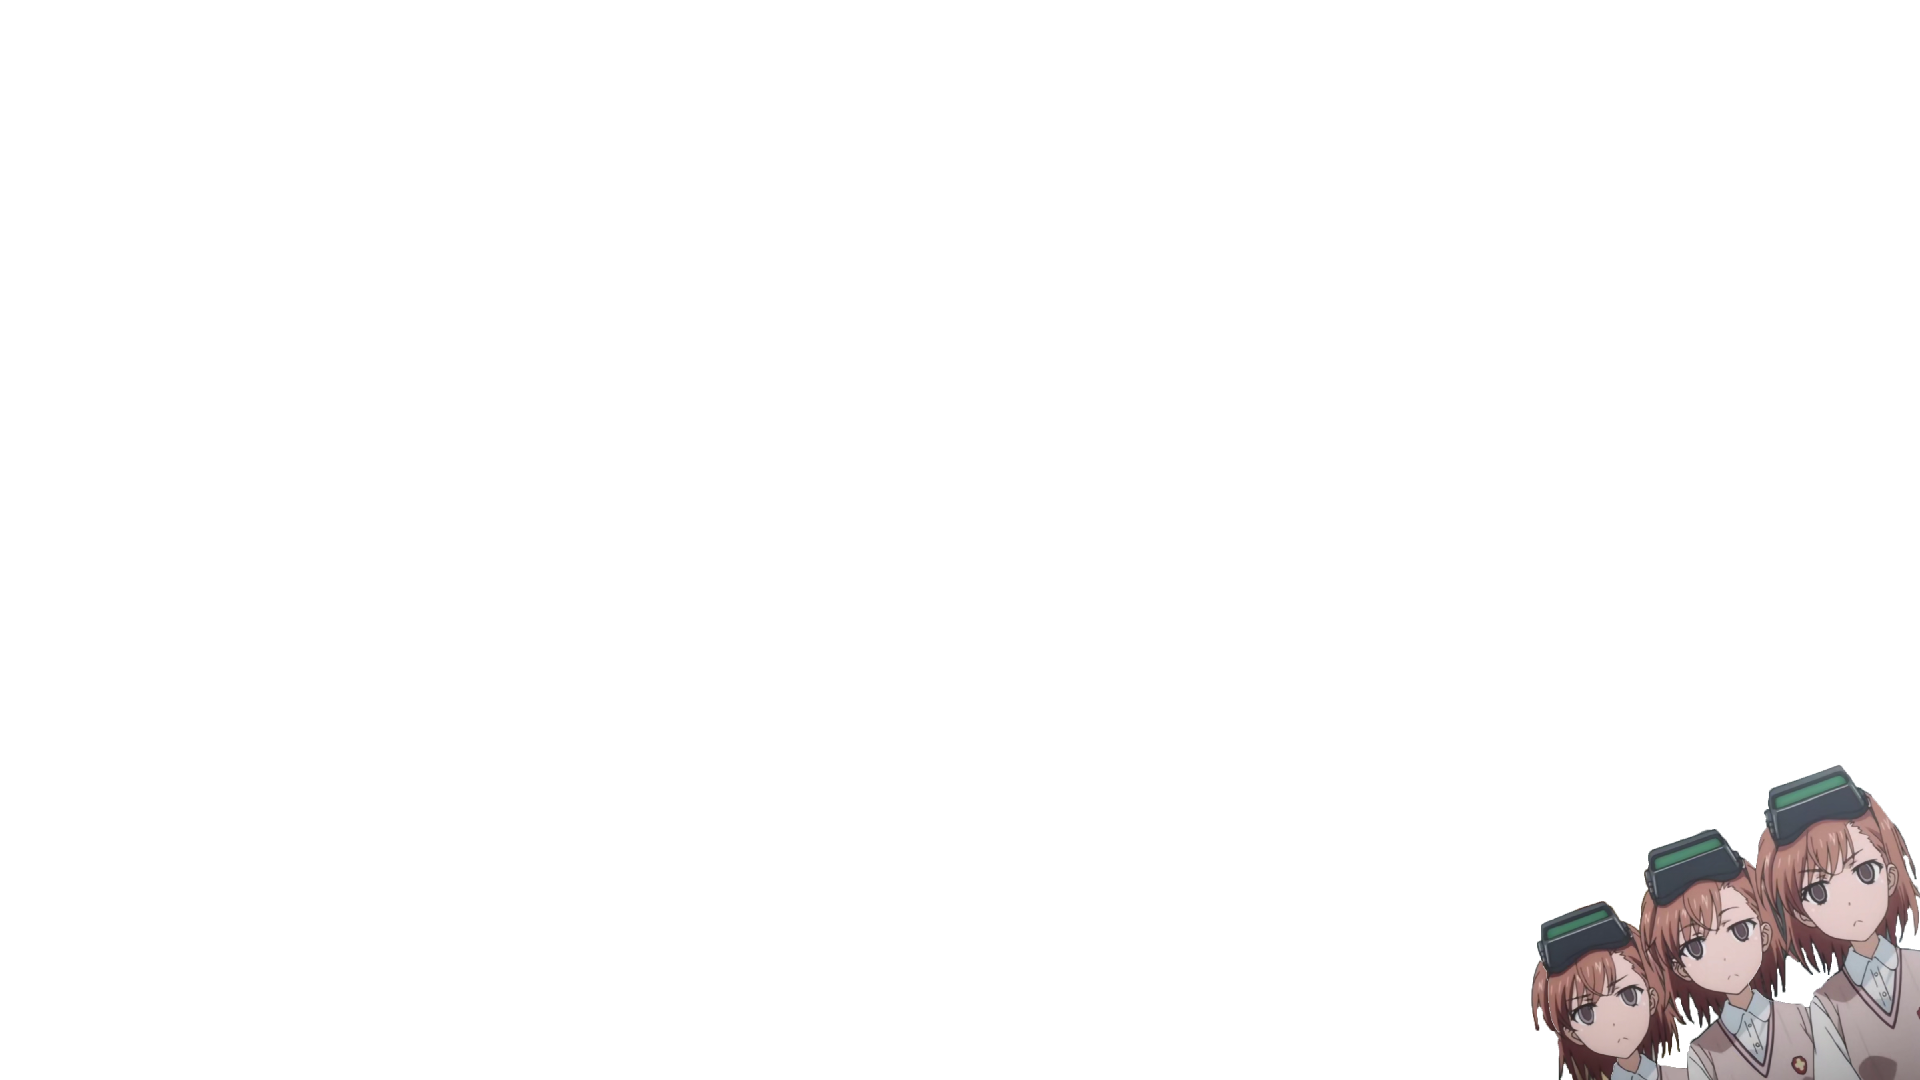
\includegraphics[height=\paperheight]{figures/sisters1080.png}}

\makeatletter 
\renewcommand{\@thesubfigure}{\hskip\subfiglabelskip}
\makeatother

\title{程序的机器级表示:数据}
\author{施朱鸣}
\date{10月22日}

\begin{document}
    \begin{frame}
        % \frametitle{}
        \titlepage
    
    \end{frame}
    \frame{\frametitle{Outline}\tableofcontents[hideallsubsections]}

    \section{数组}

    \begin{frame}[fragile]
        \frametitle{内存分配}
    
        \begin{lstlisting}
char string[12];
int val[5];
T A[L];
T* p = new T[L];
        \end{lstlisting}

        在内存中分配\(L\times sizeof(T)\)bytes的连续空间。
        
        数据类型是给编译器看的,分配的空间并没有记录自己的数据类型。
    
    \end{frame}

    \begin{frame}
        \frametitle{数组元素访问}
    
        可以用[]和指针运算来访问,C语言指针计算会自动调整跨度

        汇编会使用之前介绍过的寻址公式\(Imm(r_b,r_i,s)\)\footnote{可以复习书121页}

        \begin{figure}
            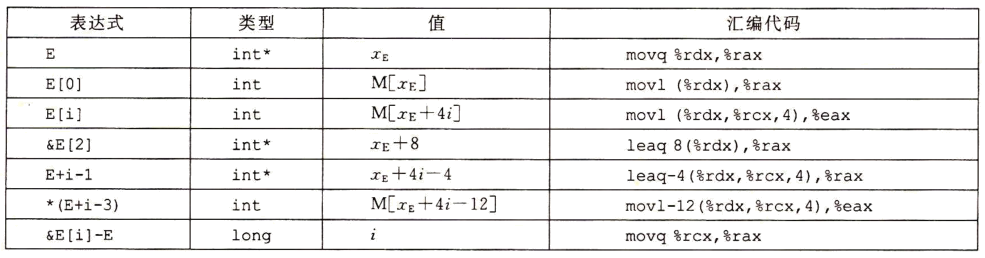
\includegraphics[width=\textwidth]{figures/elements2.png}
            % \caption{访问数组元素的方法}
        \end{figure}
    
    \end{frame}

    \begin{frame}
        \frametitle{多维数组}
    
        \[\left(
            \begin{matrix}
            A[0][0]&\cdots&A[0][C-1]\\
            \vdots&&\vdots\\
            A[R-1][0]&\cdots&A[R-1][C-1]\\
        \end{matrix}
        \right)\]

        在内存中被拉直,靠前的维度优先安排(先行后列)连续排列。
        \begin{figure}
            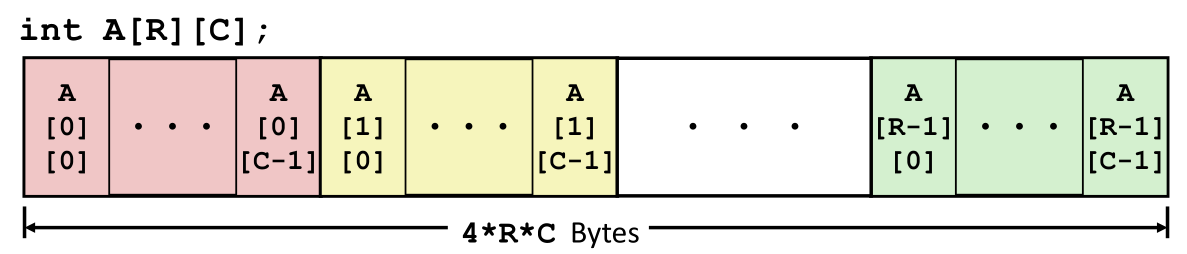
\includegraphics[width=\textwidth]{figures/multiarray.png}
        \end{figure}
    
    \end{frame}

    \begin{frame}
        \frametitle{多维数组的访问}
    
        对于\(A[i][j]\),公式为
        \[A+i\times (C\times K)+j\times K\]
        编译器利用寻址公式计算的具体方法根据优化情况而定,下面是一个例子
    \end{frame}

    \begin{frame}[fragile]
        \frametitle{多维数组的访问效率}
    
        \begin{lstlisting}
// multiarray.c
int a[2][2] = {1,1,1,1};
void ij() {
    for (int i = 0; i < 2; i++)
        for (int j = 0; j < 2; j++)
            a[i][j]++;
}
void ji() {
    for (int j = 0; j < 2; j++)
        for (int i = 0; i < 2; i++)
            a[i][j]++;
}
        \end{lstlisting}
    
    \end{frame}

    \begin{frame}
        \frametitle{多维数组的访问效率}
    
        gcc -Og -S multiarray.c 发现指令相同,猜测与优化程度、内存管理相关
        \begin{figure}
            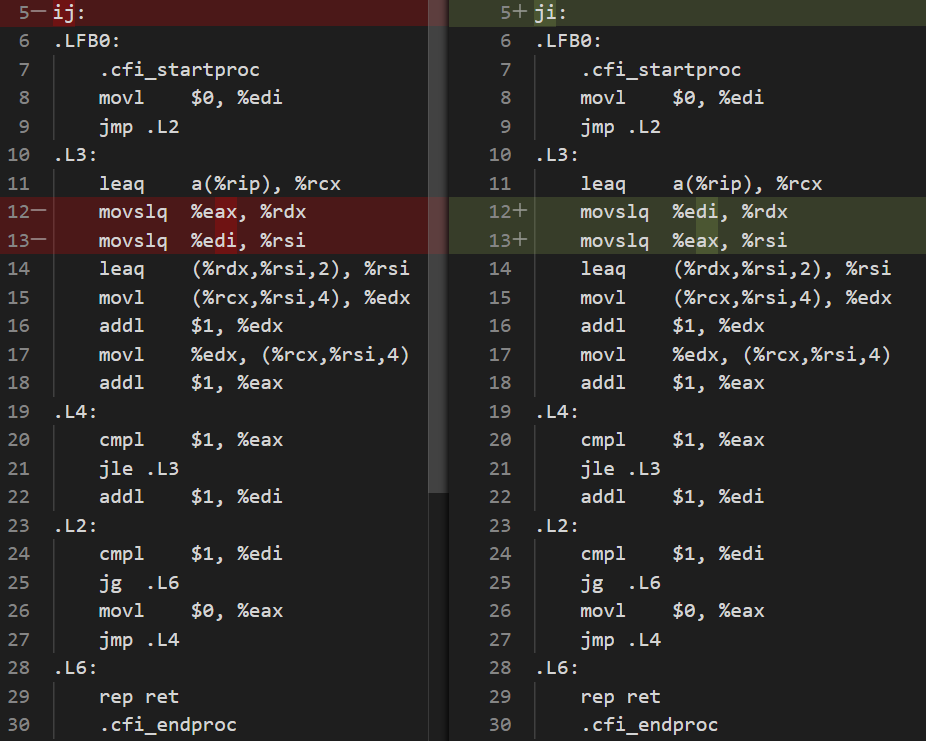
\includegraphics[height=.7\paperheight]{figures/ij.png}
        \end{figure}
    
    \end{frame}

    \begin{frame}
        \frametitle{多层数组}
    
        其实就是指针数组,访问第\(n\)层的元素需要访问\(n\)次内存,时间效率低

        \begin{figure}
            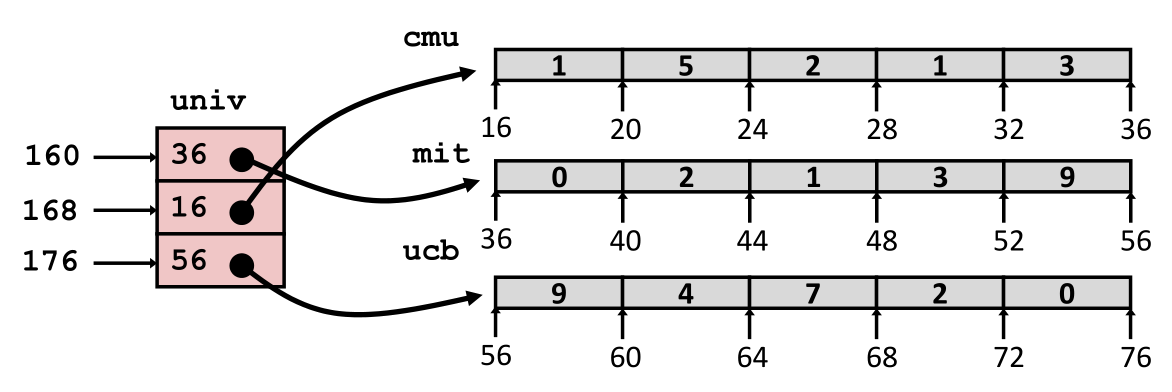
\includegraphics[width=\textwidth]{figures/multilevel.png}
        \end{figure}
    
    \end{frame}

    \begin{frame}
        \frametitle{从定长数组到变长数组}
    
        固定维度数组:编译器知道数组每个维度的大小\(C\)
        \[A+i\times (C\times K)+j\times K\]
        编译的时候就把\(C\times K\)算好了
        \begin{figure}
            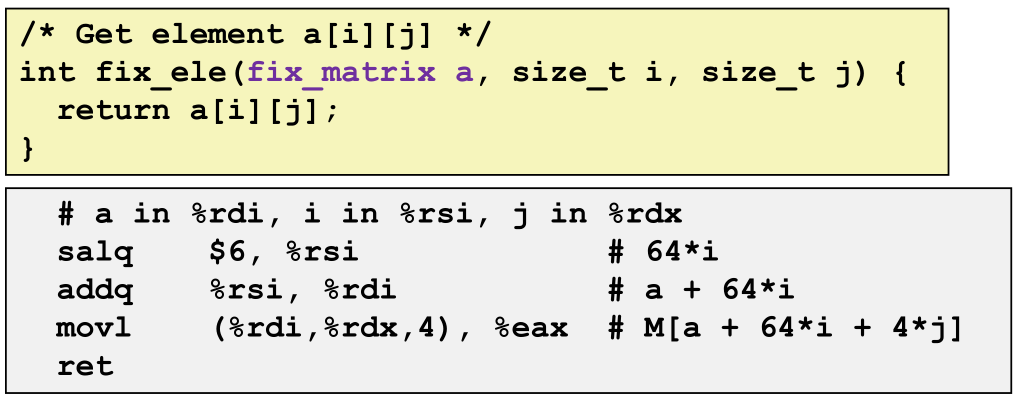
\includegraphics[width=.8\textwidth]{figures/fixed.png}
        \end{figure}
    
    \end{frame}

    \begin{frame}
        \frametitle{从定长数组到变长数组}
    
        固定维度数组:每个维度的大小\(C\)在运行时根据传入的参数确定
        \[A+i\times (C\times K)+j\times K\]
        \textbf{\(C\times K\)只能在运行时计算},时间开销更大。
% 
        当然,数组本身的连续内存空间大小还是确定的。元素的大小\(K\)也是确定的。
% 
        % 这种方法也
        只是拓展了这个函数的适用性
        % 而已
        。
        \begin{figure}
            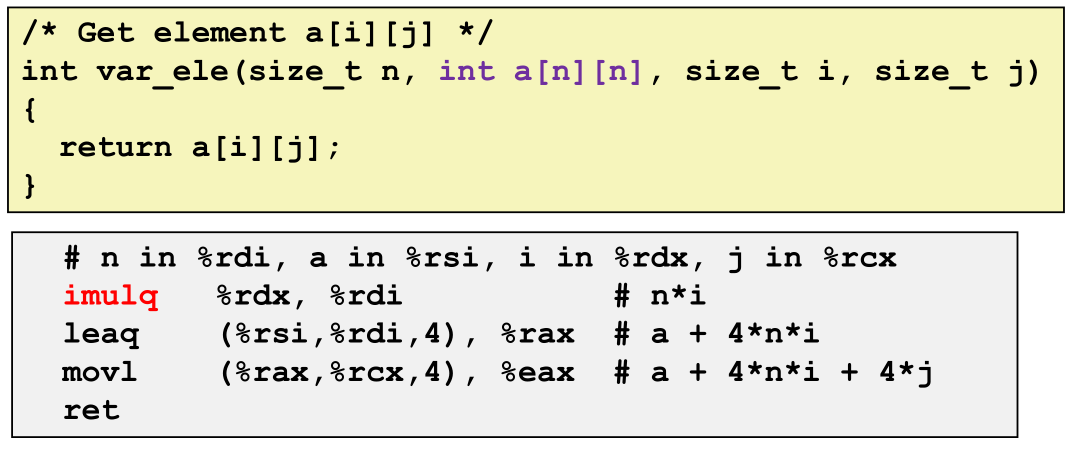
\includegraphics[width=.8\textwidth]{figures/var.png}
        \end{figure}
    
    \end{frame}

    \begin{frame}[fragile]
        \frametitle{正确理解“变长”}
    
        \begin{lstlisting}
// vararray.c
# include<stdio.h>
int main(){
    int n, p[n];
    scanf("%d",&n);
    int q[n];
    printf("p:%lu and q:%lu",sizeof(p),sizeof(q));
    return 0;
}
        \end{lstlisting}

        > gcc vararray.c \&\& echo 3 | ./a.out`

        > p:131068 and q:12
    
    \end{frame}

    \section{结构体}

    \begin{frame}
        \frametitle{结构体的定义}
    
        按照声明的顺序,各元素顺序排列在一片连续的内存空间中

        空间的大小由编译决定,机器级访问的方法类似于数组元素的访问,通过指针计算

        \begin{figure}
            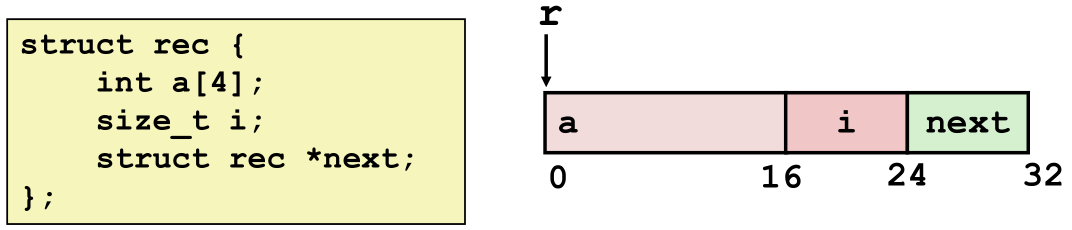
\includegraphics[width=.8\textwidth]{figures/strcut.png}
        \end{figure}
    
    \end{frame}

    \begin{frame}
        \frametitle{结构体的对齐}
    
        对齐的规则:
        \begin{itemize}
            \item 结构体内部对齐:每个K字节的基本对象的地址必须是K的倍数
            \item 结构体整体对其:结构体整体长度是结构体中最大的元素长度的整数倍
        \end{itemize}

        编译器会用0补足空隙,保证对齐

        \begin{figure}
            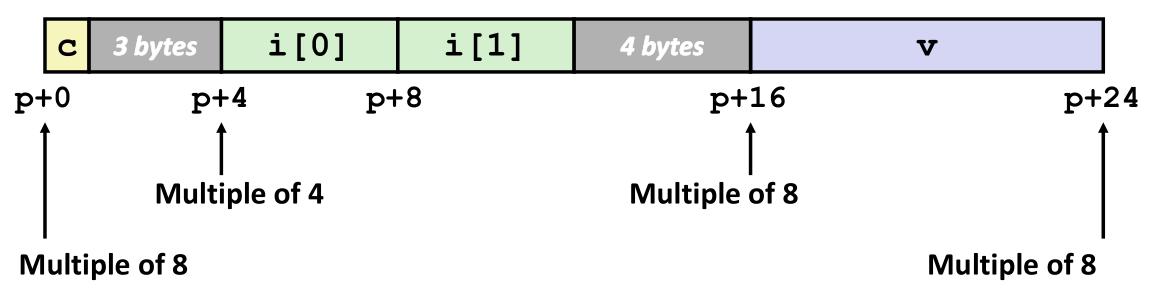
\includegraphics[width=.8\textwidth]{figures/align.png}
        \end{figure}
    
    \end{frame}

    \begin{frame}
        \frametitle{结构体元素的访问}
    
        \textbf{以不变应万变}:指针运算,遇到对齐补的0记得跳过

        \begin{figure}
            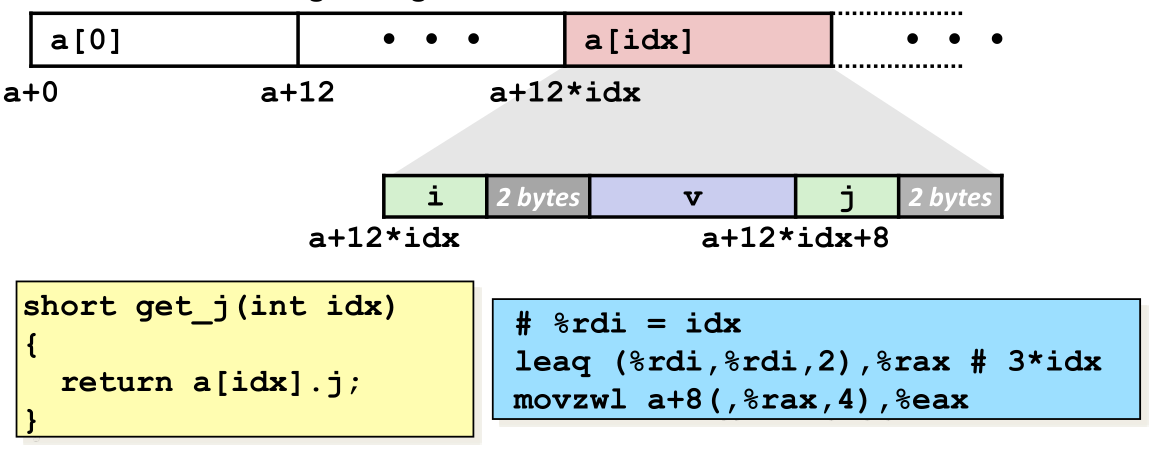
\includegraphics[width=.8\textwidth]{figures/visit.png}
        \end{figure}
    
    \end{frame}

    \begin{frame}
        \frametitle{结构体存储的优化}
    
        根据对其规则调整结构体元素的顺序

        \begin{figure}
            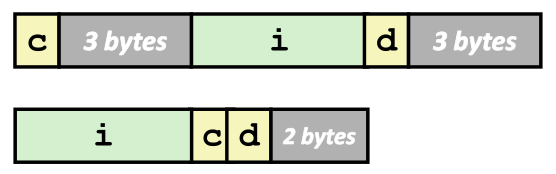
\includegraphics[width=.618\textwidth]{figures/small.png}
        \end{figure}

    
    \end{frame}

    \section{浮点数}

    \begin{frame}
        \frametitle{浮点寄存器XMM}
    
        \begin{itemize}
            \item 一共16个,每个16 bytes,命名为\%xmm0到\%xmm15
            \item 不止可以存浮点数,也不止可以放一个数
        \end{itemize}

        \begin{figure}
            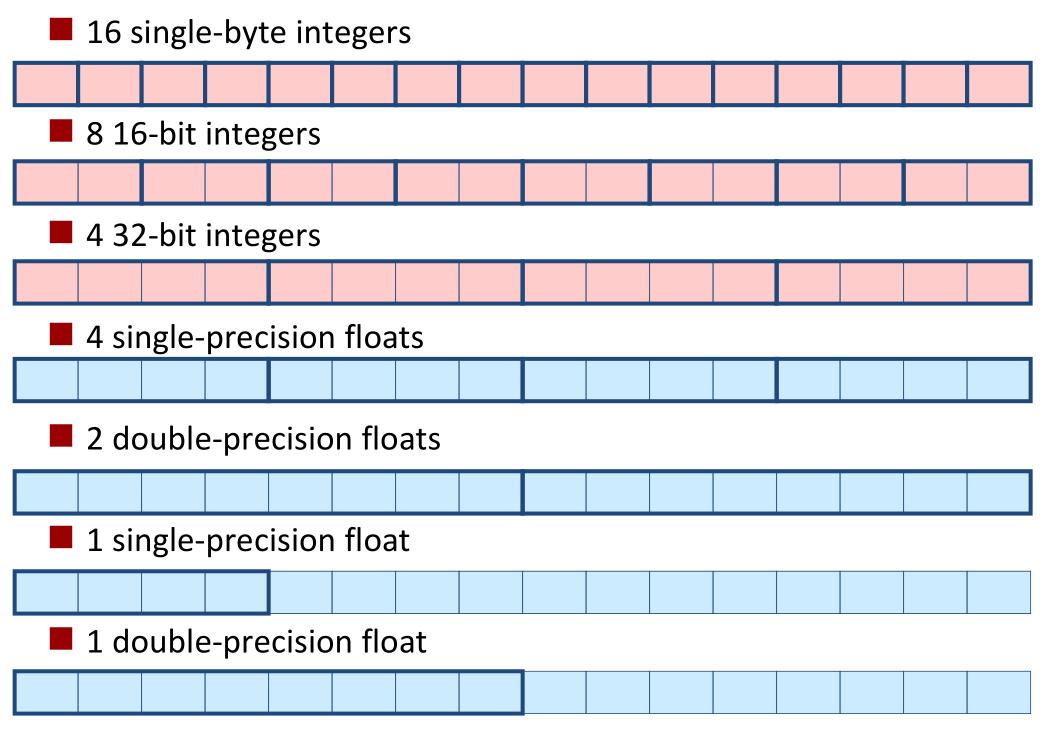
\includegraphics[height=.6\paperheight]{figures/xmm.png}
        \end{figure}
    
    \end{frame}

    \begin{frame}
        \frametitle{浮点计算指令}
    
        \begin{figure}
            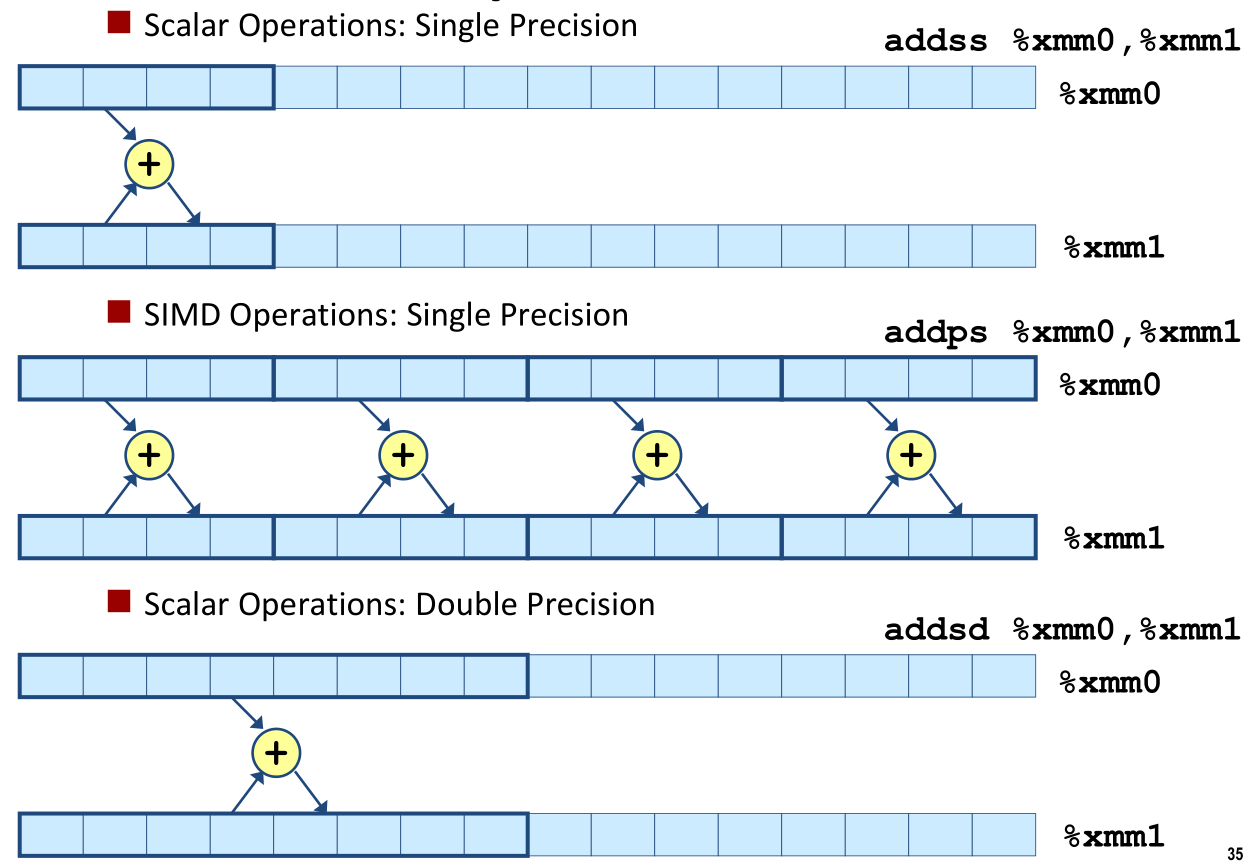
\includegraphics[width=.7\textwidth]{figures/fpu.png}
        \end{figure}
    
    \end{frame}

    \begin{frame}
        \frametitle{全部浮点数参数时的传参}
    
        规则可以类比非浮点的计算
        \begin{itemize}
            \item 参数依次放入\%xmm0,\%xmm1等
            \item 返回值放入\%xmm0到
            \item \textbf{所有的xmm寄存器都是caller-saved}
        \end{itemize}

        如果有非浮点参数和返回值呢?
        \pause

        非浮点的参数用普通寄存器依次存放,浮点的参数用\%xmm依次存放。

        xmm寄存器之间的移动和内存与xmm的移动有浮点运算的一套指令
    
    \end{frame}

    \begin{frame}
        \frametitle{浮点相关的移动指令\footnote{教材206页}}
    
        把指令前面的v去掉。其他浮点运算指令见书上210页。
        \begin{figure}
            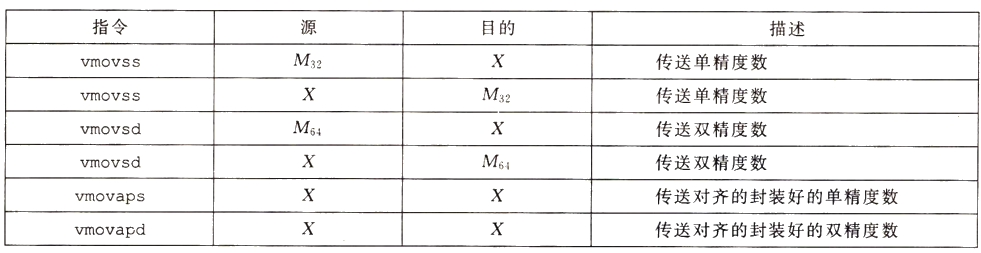
\includegraphics[width=\textwidth]{figures/vmov.png}
        \end{figure}
    
    \end{frame}

    \section{练习}

    \begin{frame}
        \frametitle{练习题3.38}
    
        \begin{figure}
            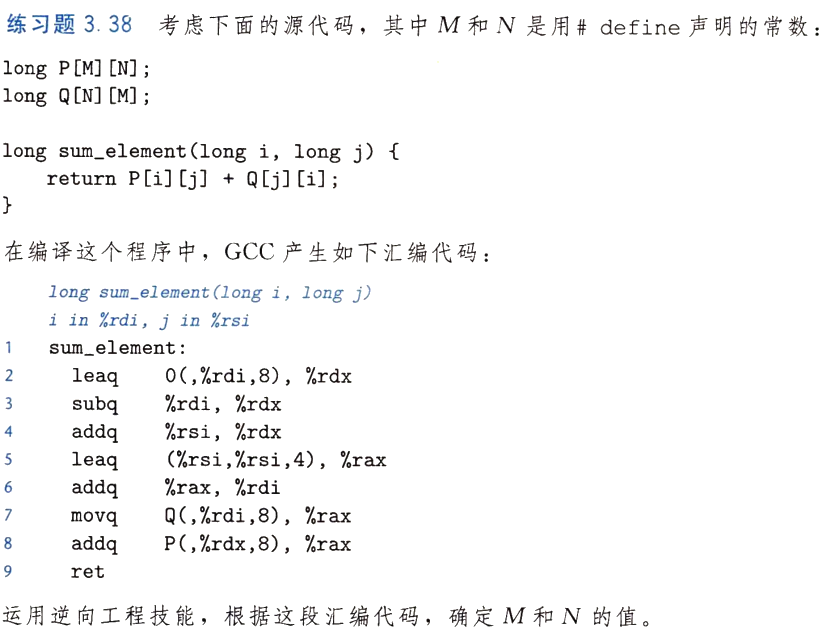
\includegraphics[width=.7\textwidth]{figures/338.png}
        \end{figure}
    
    \end{frame}

    \begin{frame}
        \frametitle{练习题3.44}
    
        \begin{figure}
            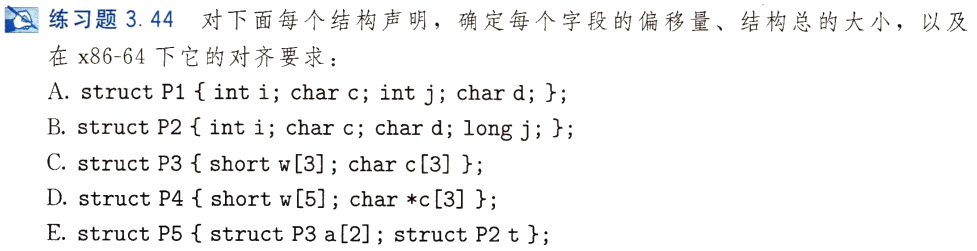
\includegraphics[width=.8\textwidth]{figures/344.png}
        \end{figure}
    
    \end{frame}

    \section*{致谢}

    \begin{frame}
        \frametitle{致谢}
        LaTeX代码开源在https://github.com/ShiZhuming/pku-ics

        祝大家写lab顺利,谢谢聆听!
    
    \end{frame}
    
\end{document}